\section{Conformance Checking}
Conformance check tries to verify if the behavior of a process model is in line with the behavior recorded in an event log.
It identifies execution traces in the event log that deviate from the process model and vice versa.
There are several techniques to perform conformance checking.

%#TODO: I would eliminate this paragraph 
\paragraph{Usage of Conformance Checking:}
Conformance checking can be used for several purposes:
\begin{itemize}
    \item \textbf{Discriminate} between fitting and non-fitting traces;
    \item \textbf{Locate Deviations} within traces;
    \item \textbf{Compare Models:} different process models can be compared based on their conformance with an event log;
    \item \textbf{Diagnonistics:} identify bottlenecks and inefficiencies in the process by analyzing deviations;
    \item \textbf{Compare discovered models:} evaluate the quality of process discovery algorithms by measuring how well the discovered model fits the event log;
\end{itemize}

\subsection{Replay-based Conformance Checking}
Replay-based conformance checking techniques try to replay the traces recorded in an event log on a process model.
During the replay, information about deviations are collected:
\begin{itemize}
    \item \textbf{Produced Tokens $p$:} the count of tokens produced during the replay of a trace. In the beginning, a token will be produced for the source place;
    \item \textbf{Consumed Tokens $c$:} the count of tokens consumed during the replay of a trace. At the end, a token will be consumed for the sink place;
    \item \textbf{Missing Tokens $m$:} When an activity is executed in the event log, but the corresponding transition in the process model cannot be fired due to missing tokens;
    \item \textbf{Remaining Tokens $r$:} After replaying a trace, the tokens that are left in the process model;
\end{itemize}
Using these statistics, we can define the fitness of a trace as follows:
\begin{equation}
    \label{eq:fitness}
    Fitness = \frac{1}{2}(1 - \frac{m}{c}) + \frac{1}{2} (1 - \frac{r}{p})
\end{equation}
This measure yields a value between 0 and 1, that can be interpreted as the percentage of behavior in the event log that can be explained by the process model.
\paragraph{Fitness of an Event Log}
The fitness equation \ref{eq:fitness} can be used to calculate the fitness of a single trace.
We can extend this to calculate the fitness of an entire event log by calculating by summing the fitness of each trace, weighted by the number of times the trace appears in the event log:
\begin{equation}
    \label{eq:logfitness}
    Fitness_{Log} = \frac{1}{2} (1 - \frac{\sum_{t \in L} m(t)}{\sum_{t \in L} c(t)}) + \frac{1}{2} (1 - \frac{\sum_{t \in L} r(t)}{\sum_{t \in L} p(t)})
\end{equation}
%#TODO: I would eliminate this paragraph 
\paragraph{Pros and Cons:}
Replay-based conformance checking has several advantages:
\begin{itemize}
    \item Able to differentiate between fitting and non-fitting behavior;
    \item intuitive and easy to understand;
    \item efficient to compute for any log;
\end{itemize}
However, there are also some drawbacks:
\begin{itemize}
    \item The fitness for problematic traces may still be high, making it difficult to identify specific deviations;
    \item Only defined for Petri nets;
    \item It doesn't allow to locate the exact position of deviations within a trace;
\end{itemize}

\subsection{Alignment-based Conformance Checking}
Alignment-based conformance checking is built upon the weaknesses of replay-based conformance checking.
In fact, replay-based techniques cannot provide a corresponding path in the process model.
\\The idea of alignment-based conformance checking is to find the best possible alignment between a trace in the event log and a corresponding path in the process model.
An alignment is a sequence of steps that map events in the trace to transitions in the process model.
Each step in the alignment can be one of the following:
\begin{itemize}
    \item \textbf{Synchronous Move:} an event in the trace matches a transition in the process model;
    \item \textbf{Log Move:} an event in the trace does not have a corresponding transition in the process model;
    \item \textbf{Model Move:} a transition in the process model is executed without a corresponding event in the trace;
\end{itemize}
It's an \textbf{illegal} move to two different events between the log and the model.
\\\\Then we define a \textbf{standard cost} function to assign costs to each type of move:
\begin{itemize}
    \item \textbf{Synchronous Move:} cost 0;
    \item \textbf{Log Move:} cost 1;
    \item \textbf{Model Move:} cost 1;
\end{itemize}
The goal of alignment-based conformance checking is to find the alignment with the lowest total cost, which is defined as the \textbf{optimal alignment}.
\begin{figure}[H]
    \centering
    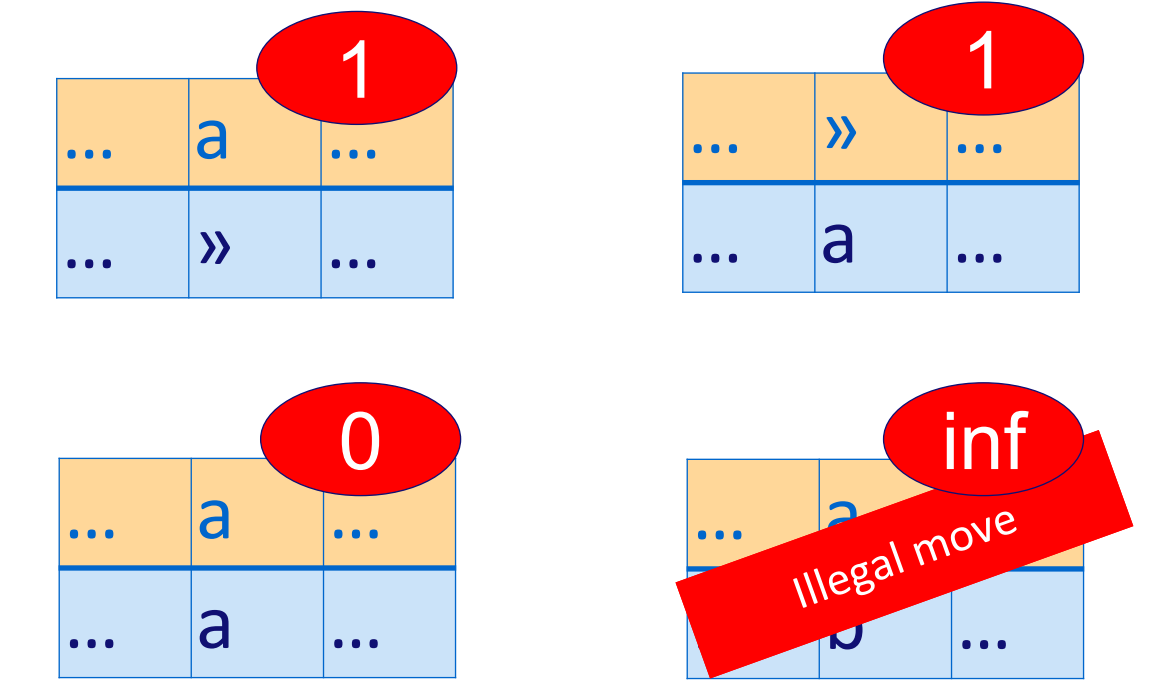
\includegraphics[width=0.6\textwidth]{../images/conformance_checking/alignment.png}
    \caption{Example of an alignments}
\end{figure}
It's possible to define various cost functions depending on the specific application or domain, or to assign different weights to different types of moves.

\subsubsection*{Computing Fitness}
The idea is to compare the cost of an optimal alignment with the cost of a worst-case alignment.
In formula:
\begin{equation}
    fitness(\sigma, N) = 1 - \frac{\delta(\lambda_{opt}(\sigma, N))}{\delta(\lambda_{worst}(\sigma, N))}
\end{equation}
Where:
\begin{itemize}
    \item $\sigma$ is the trace in the event log;
    \item $N$ is the process model;
    \item $\delta$ is the cost function;
    \item $\lambda_{opt}(\sigma, N)$ is the optimal alignment between the trace and the process model;
    \item $\lambda_{worst}(\sigma, N)$ is the worst-case alignment between the trace and the process model;
\end{itemize}
The \textbf{worst-case} alignment can be easily calculated by performing a complete sequence of log moves to represent the entire trace, followed by a series of model moves to traverse the shortest path from the initial state to the final state.
\\\\In order to compute the fitness of an entire event log, we can extend the previous formula by summing the fitness of each trace, weighted by the number of times the trace appears in the event log:
\begin{equation}
    fitness(L, N) = 1 - \frac{\sum_{\sigma \in L} L(\sigma) \times \delta(\lambda_{opt}(\sigma, N))}{\sum_{\sigma \in L} L(\sigma) \times \delta(\lambda_{worst}(\sigma, N))}
\end{equation}
where $L(\sigma)$ is the frequency of $\sigma$ on the log $L$.
Otherwise you can also use this formula, computing the fitness of each trace and then averaging it:
\begin{equation}
    fitness(L, N) = \frac{\sum_{\sigma \in L} L(\sigma) \times fitness(\sigma, N)}{\sum_{\sigma \in L} L(\sigma)}
\end{equation}